\section{Redis}
\subsection{Allgemeines}
\begin{itemize}
    \item Schemafrei
    \item Daten werden grundsätzlich In-Memory (Schnell!) gespeichert \& können wahlweise auch auf die Festplatte übertragen werden
    \item Zu einem gewissen Key können ein oder mehrere Werte abgespeichert werden
    \item Eventual Consistency $\implies$ Daten werden nicht sofort auf allen Servern/Partitionen geschrieben, sondern erst nach einer gewissen Zeit
    \begin{itemize}
        \item Dadurch kann es bei gleichen Abfragen teilweise zu unterschiedlichen Ergebnissen kommen!
    \end{itemize}
    \item Transaktionen $\implies$ Optimistic Locking $\implies$ Alle User haben Lesezugriff, im Falle einer Änderung werden alle benachrichtigt
\end{itemize}

\subsection{Sharding}
\begin{itemize}
    \item Auch bekannt als Partitioning $\implies$ Die Daten werden anhand ihrer Keys aufgeteilt und dann auf verschiedenen Maschinen gespeichert
\end{itemize}

\subsection{Replication}
\begin{itemize}
    \item Die Daten werden über mehrere Maschinen hinweg gespiegelt $\implies$ Erhöht Lesegeschwindigkeit
\end{itemize}

\subsection{Cluster}
\begin{itemize}
    \item Daten können auf mehrere Nodes aufgeteilt werden; Es kann weitergearbeitet werden, wenn Nodes ausfallen
    \item Für jede Node im Cluster muss ein Config-File erstellt werden, welches wie folgt aussieht (Ports müssen entsprechend angepasst werden):
\end{itemize}
\begin{figure}[H]
    \centering
    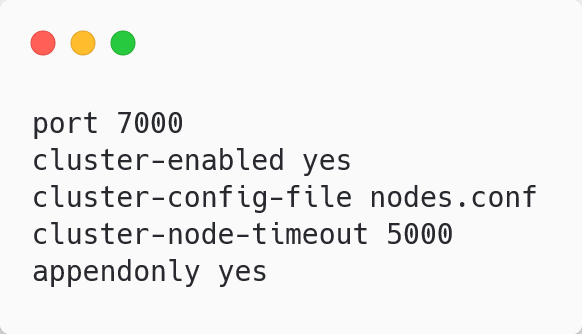
\includegraphics[scale=.3]{res/themenkorb_8/redis_cluster_config.png}
\end{figure}

\subsubsection{Weitere Konfigurationsparameter}
\begin{itemize}
    \item \textbf{cluster-slave-validity-factor}: Gibt, multipliziert mit cluster-node-timeout, die maximale Zeit an, in der der Slave versucht für den Master zu übernehmen
    \begin{itemize}
        \item Wenn 0 $\implies$ Slave probiert immer, Master zu ersetzen
    \end{itemize}
    \item \textbf{cluster-migration-barrier}: Minimum an Slaves, die einem Master erhalten bleiben müssen und somit nicht zu anderen Masters migriert werden können
    \item \textbf{cluster-require-full-coverage}: Gibt an, ob die gesamte Slot-Range durch einen Master gecovered sein muss
\end{itemize}

\subsubsection{Data Sharding}
\begin{itemize}
    \item Ein Redis-Cluster enthält 16484 Hash-Slots (Keys werden nach Formel dem Slot zugewiesen)
    \item Jede Node ist für einen gewissen Teil dieser Hash-Slots zuständig
    \item Multiple Key Operations $\implies$ Alle Keys müssen Teil des selben Hash-Slots sein!
\end{itemize}

\subsubsection{Master \& Slave}
\begin{itemize}
    \item Um Ausfallssicherheit zu garantieren $\implies$ Ein Master kann N Slaves haben, welche die gleiche Hash-Slot-Range abdecken!
    \item Node Timeout gibt an, wie lange gewartet wird, bis eine Node als inaktive gilt \& ein Slave übernimmt
\end{itemize}

\subsection{Befehle}
\subsubsection{Standard}
\begin{figure}[H]
    \centering
    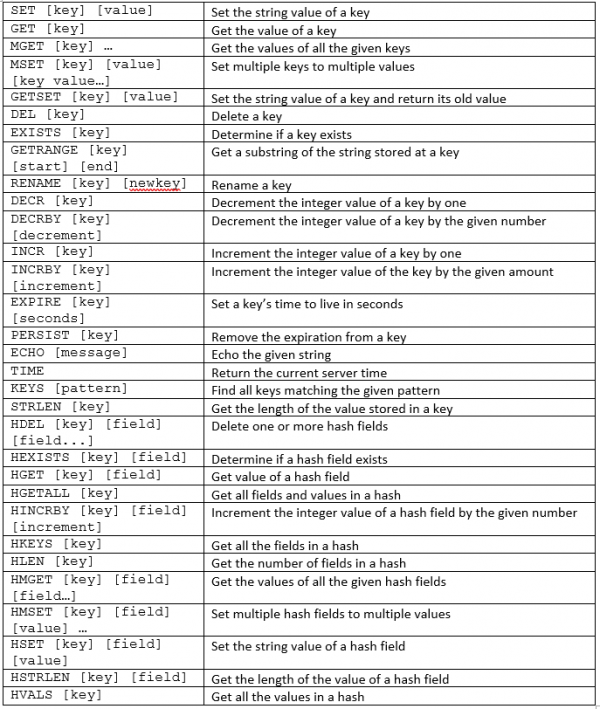
\includegraphics[scale=.8]{res/themenkorb_8/importantcommands_redis.png}
\end{figure}
\subsubsection{Geo}
\begin{figure}[H]
    \centering
    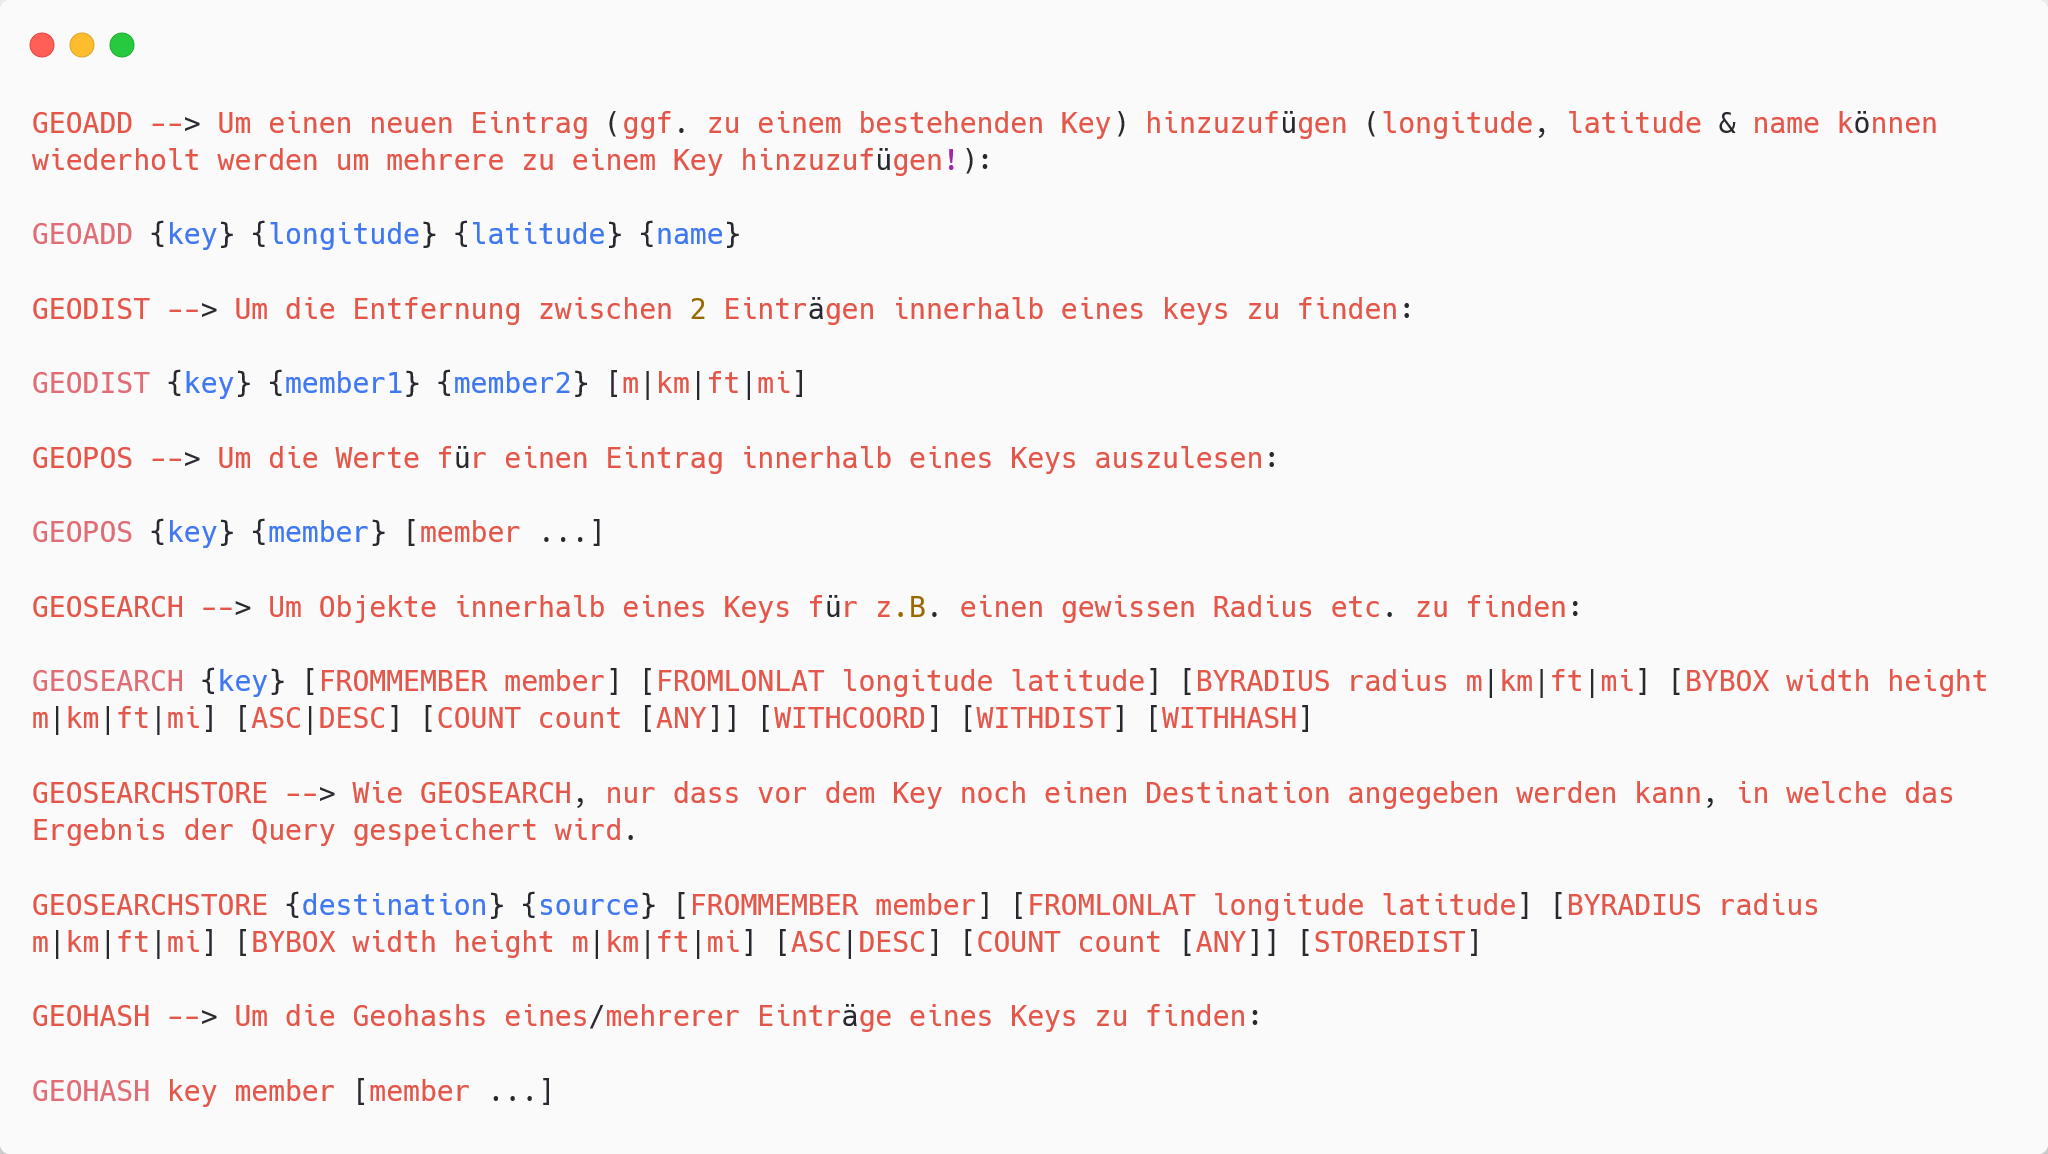
\includegraphics[width=\textwidth]{res/themenkorb_8/redis_geo.png}
\end{figure}